\documentclass[12pt]{article}
\usepackage{amsmath,amssymb}
\usepackage{graphicx}
\begin{document}

\section*{Question 2}

Let $f : \mathbb{R} \to (1, +\infty)$ be defined by $f(x) = e^x + 1$.

\subsection*{1. Show that $f$ is a bijection}

\paragraph{Injectivity:}
Suppose $f(a) = f(b)$ for some $a, b \in \mathbb{R}$. Then
\[
  e^a + 1 = e^b + 1 
  \quad \Longrightarrow \quad
  e^a = e^b 
  \quad \Longrightarrow \quad
  a = b.
\]
Therefore, $f$ is injective.

\paragraph{Surjectivity:}
The codomain of $f$ is $(1, +\infty)$. For any $y > 1$, we want to find an $x \in \mathbb{R}$ such that $f(x) = y$. That is,
\[
  e^x + 1 = y 
  \quad \Longrightarrow \quad
  e^x = y - 1 
  \quad \Longrightarrow \quad
  x = \ln(y - 1).
\]
Since $y - 1 > 0$, $\ln(y - 1)$ is well-defined for all $y>1$. Hence every $y$ in $(1,+\infty)$ has a preimage in $\mathbb{R}$. This proves surjectivity.

Combining injectivity and surjectivity shows that $f$ is \textbf{bijective}.

\subsection*{2. Find the inverse function $f^{-1}$}

Starting with $y = e^x + 1$, we solve for $x$:
\[
  y - 1 = e^x
  \quad \Longrightarrow \quad
  x = \ln(y - 1).
\]
Therefore, the inverse function is
\[
  f^{-1}(y) = \ln\bigl(y - 1\bigr), 
\]
with domain $(1,+\infty)$ and range $\mathbb{R}$.

\subsection*{3. Plot the curves of $f$ and $f^{-1}$ in the same graph}

\begin{itemize}
\item The function $f(x) = e^x + 1$ is an exponential curve shifted upward by 1, with a horizontal asymptote at $y = 1$.
\item The inverse $f^{-1}(y) = \ln(y - 1)$ is a logarithmic curve shifted to the right by 1, with a vertical asymptote at $y = 1$ (when plotted in the $xy$-plane, this asymptote is at $x = 1$ if we interchange the roles of $x$ and $y$).
\item When both are graphed in the same coordinate plane (treating $f^{-1}$ as a function of $x$), the two curves are symmetric with respect to the line $y = x$.
\end{itemize}

\begin{figure}[ht]
  \centering
  \begin{minipage}[t]{0.45\textwidth}
    \centering
    % Replace "e^x+1.jpg" with your actual file name
    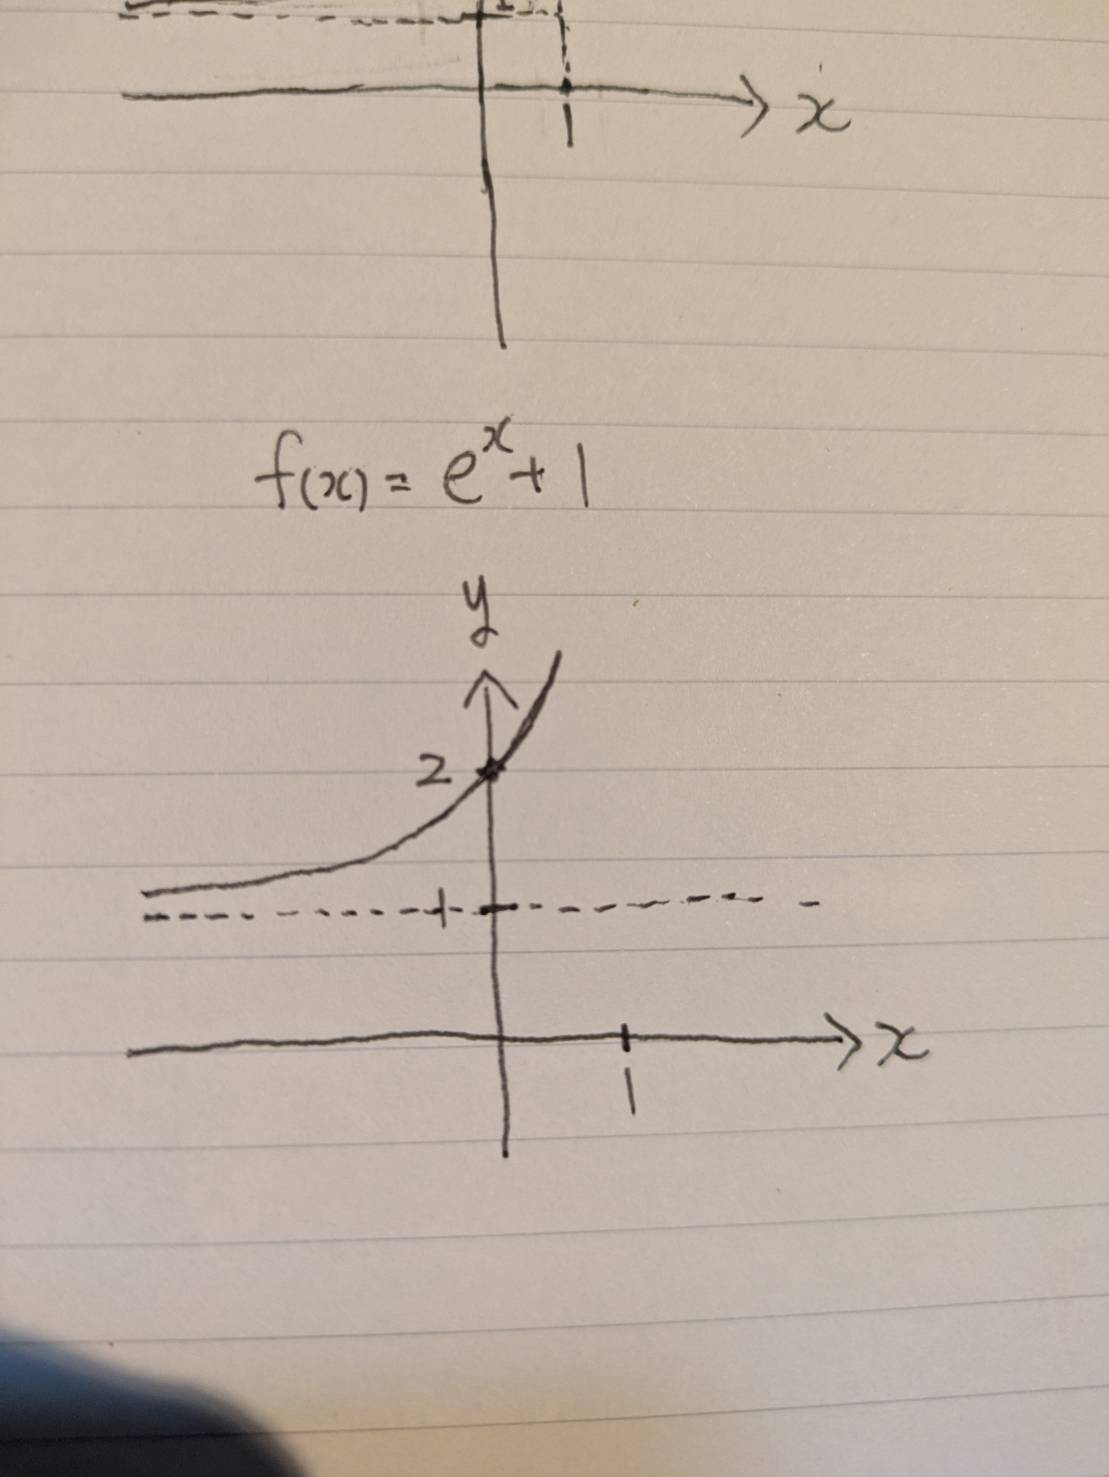
\includegraphics[width=\textwidth]{images/e^x+1.jpg}
    \caption{Graph of $f(x) = e^x + 1$.}
    \label{fig:exp-plus-1}
  \end{minipage}
  \hfill
  \begin{minipage}[t]{0.45\textwidth}
    \centering
    % Replace "ln(y-1).jpg" with your actual file name
    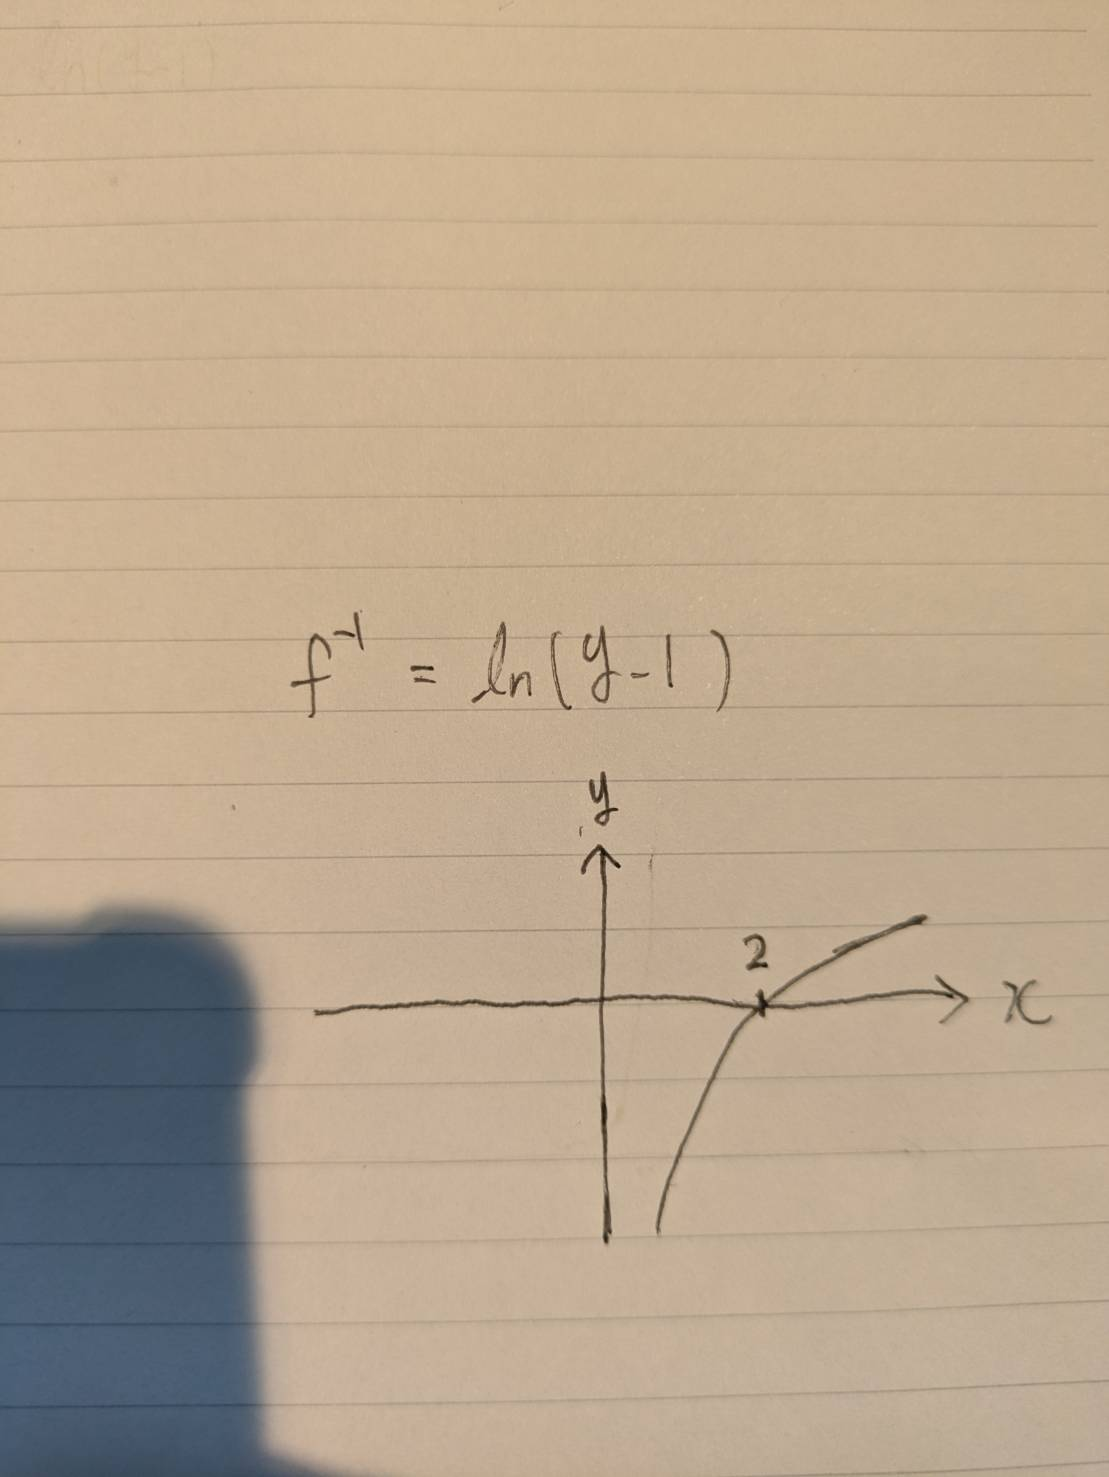
\includegraphics[width=\textwidth]{images/ln(y-1).jpg}
    \caption{Graph of $f^{-1}(x) = \ln(x - 1)$.}
    \label{fig:ln-of-x-minus-1}
  \end{minipage}
\end{figure}

\subsection*{4. What can be said about these two curves?}

They are reflections of each other across the line $y = x$. This is a characteristic relationship between any bijective function and its inverse. The domain of $f$ is all real numbers, and its range (which is $(1,+\infty)$) becomes the domain for $f^{-1}$. Conversely, the range of $f^{-1}$ is $\mathbb{R}$, matching the original domain of $f$.

\end{document}
